\section{Алгоритм, основанный на пересечении языков}

В качестве единого подхода к построению частичных решений для задачи CFPQ был выбран алгоритм~\cite{Chaudhuri08, Orachev20}, основанный на пересечении языков. Причина выбора именно этого решения следующая: в основе остальных подходов лежат алгоритмы парсинга, все из которых имеют кубическое время работы и неизвестно, могут ли быть ускорены, тогда как данный подход основан на графовых алгоритмах (а именно, на решении задачи построения инкрементального транзитивного замыкания), засчёт чего более подвержен модификациям.

% Конечный автомат
% \begin{definition}
  % \textit{Мы считаем, что читатель знаком с понятием конечного автомата, если нет, пусть идёт знакомиться с книгой Ахо, Хопкрофта и Ульмана}
% \end{definition}

\subsection{Сведение к задаче достижимости для РКА}

% В данном разделе будет подробно описан алгоритм, предложенный в~\cite{Orachev20}, в модификации которого будет состоять дальнейшая работа.

Главной идеей алгоритма является следующее замечание: любой помеченный граф $G$ можно рассматривать как \textit{недетерминированный конечный автомат}, в котором не обозначены начальное и конечные состояния.

% Конечный автомат
\begin{definition}
  % \textit{Мы считаем, что читатель знаком с понятием конечного автомата, если нет, пусть идёт знакомиться с книгой Ахо, Хопкрофта и Ульмана}

  \textit{Недетерминированный конечный автомат (или НКА)}\footnote{Nondeterministic finite automaton (или NFA)}~--- это пятёрка $\q{Q, \Sigma, \delta, q_0, F}$:
  \vspace{-\topsep}
  \begin{itemize}
    \setlength\itemsep{-0.1em}
    \item $Q$~--- конечное множество состояний
    \item $\Sigma$~--- конечный алфавит
    \item $\delta \colon Q \times \Sigma \to 2^Q$~--- функция перехода
    \item $q_0 \in Q$~--- начальное (стартовое) состояние
    \item $T \subseteq Q$~--- множество конечных (терминальных) состояний
  \end{itemize}

  \textit{Язык, распознаваемый НКА} $\cool{A}$~--- язык $L(\cool{A})$ слов, на которых автомат, следуя функции перехода, может дойти из стартового состояние в терминальное хотя бы одним способом.

  Недетерминированные конечные автоматы задают \textit{регулярные языки}.
\end{definition}

\TODO: пример (в фигуру с автоматом $0 \path 2$)

\begin{figure}[H]
  \begin{tikzpicture}[shorten >=1pt,auto]
    \node[state, initial]   (q_0)                      {$0$};
    \node[state]            (q_1) [above right=of q_0] {$1$};
    \node[state, accepting] (q_2) [right=of q_0]       {$2$};
    \node[state]            (q_3) [right=of q_2]       {$3$};
    \path[->]
    (q_0) edge  node {$a$} (q_1)
    (q_1) edge  node {$a$} (q_2)
    (q_2) edge  node {$a$} (q_0)
    (q_2) edge[bend left, above] node {$b$} (q_3)
    (q_3) edge[bend left, below] node {$b$} (q_2);
  \end{tikzpicture}
  \caption{НКА, задающий слова, читаемые на путях $0 \path 2$.\\ Например, $aa$, $aabb$ или $aabbaaa$}
\end{figure} 

\begin{proposition}
  Если зафиксировать конкретные вершины $u$ и $v$ помеченного графа $G$ как стартовое и конечное состояния, то полученный автомат будет задавать язык слов, читаемых на путях из $u$ в $v$.

\end{proposition}

Язык, задаваемый подобным автоматом, будем обозначать как $L(G, u, v)$.

Получаем, что для каждой пары вершин $u$ и $v$, наличие пути $p \colon u \path v$, такого, что на нём читается слово $w \in L(\cool{G})$ равносильно непустоте пересечения языков $L(G, u, v)$ и $L(\cool{G})$ (действительно, в пересечении будут лежать ровно слова, выводимые грамматикой и при этом читаемые на каком-либо пути $u \path v$).

Для построения пересечения языков нам потребуется такая конструкция, как прямое произведение автоматов.

\begin{definition}[Прямое произведение автоматов]

\TODO

\end{definition}

\begin{proposition}\label{prop:reg_inter} \cite{Hopcroft1979}
  Автомат $A$, построенный как прямое произведение автоматов $A_1$ и $A_2$ ($A = A_1 \otimes A_2$), распознаёт язык, равный пересечению языков $A_1$ и $A_2$ ($\cool{L}(A) = \cool{L}(A_1) \cap \cool{L}(A_2)$)
\end{proposition}

Заметим, однако, что лишь один из языков, чьё пересечение нам нужно, является регулярным (и, следовательно, задаётся автоматом)~--- язык входного графа. Второй же язык является контекстно-свободным и недетерминированный конечным автоматом не задаётся. Однако он задаётся с помощью более сложного автомата~--- рекурсивного. 

\begin{definition}[Рекурсивный конечный автомат (РКА)]
  \textit{Рекурсивный конечный автомат (или РКА)}\footnote{Recursive state machine}~\cite{Alur05}~--- это набор компонент $\q{M_1, M_2, \dots, M_k}$, с выделенной стартовой компонентой, где каждая компонента $M_i$~--- это пятёрка $\q{Q_i, \Sigma_i, En_i, Ex_i, \delta_i}$:
      \vspace{-\topsep}
      \begin{itemize}
        \setlength\itemsep{-0.1em}
        \item $Q_i$~--- конечное множество состояний
        \item $\Sigma_i$~--- конечный алфавит
        \item $En_i \subset Q_i$~--- множество начальных состояний
        \item $Ex_i \subset Q_i$~--- множество конечных состояний
        \item $\delta_i \colon Q_i \times (\Sigma_i \cup \bigcup\limits_{j = 1}^k En_i \times Ex_i ) \to 2^{Q_i}$~--- функция перехода. У $\delta_i$ есть два типа переходов: \textit{внутренние}, которые работают как обычные переходы в НКА и \textit{рекурсивные}, которые делают вызов другой компоненты (при этом обозначая начальную и конечную вершину в ней).
      \end{itemize}

  Неформально, это набор компонент, каждая из которых представляет собой НКА, на рёбрах которого могут быть ``рекурсивные вызовы'' других компонент.

  % Язык, задаваемый РКА $\cool{R}$~--- язык $L(\cool{R})$ слов, на которых автомат, следуя функции перехода, может дойти от начального до конечного состояния стартовой компоненты хотя бы одним способом.
\end{definition}

\TODO: пример

\begin{proposition}\cite{Alur05}
  Утверждение \ref{prop:reg_inter} остаётся верным, если один из языков задан РКА. 
\end{proposition}

При прямом произведении НКА и РКА получается также РКА. А именно, при произведении РКА $\cool{R} = \q{M_1, \dots, M_k},  M_i = \q{Q_i, \Sigma_i, En_i, Ex_i, \delta_i}$ и НКА $\cool{A} = \q{Q, \Sigma, \delta, q_0, F}$, получается РКА $\cool{P} = \cool{R} \otimes \cool{A}$, состоящий из $k$ компонент $\cool{M}_i$, таких что
  \vspace{-\topsep}
  \begin{itemize}
    \setlength\itemsep{-0.1em}
    \item множество состояний $\cool{M}_i$ равно декартову произведению $Q_i \times Q$
    \item множество начальных состояний $\cool{M}_i$ равно $En_i \times Q$
    \item множество конечных  состояний $\cool{M}_i$ равно $Ex_i \times Q$
    \item для каждого внутреннего перехода $q_s \xrightarrow{a} q_t \in \delta_i$, в $\cool{M}_i$ есть внутренние переходы $\q{q_s, u} \xrightarrow{a} \q{q_t, v}$ для всех $u, v \in Q$, что $u \xrightarrow{a} v \in \delta$
    \item для каждого внешнего перехода $\q{q_s \xrightarrow{en, ex} q_t} \in \delta_i$, в $\cool{M}_i$ есть внешние переходы $\q{q_s, q} \xrightarrow{\q{en, q}, \q{ex, q}} \q{q_t, q}$ для всех $q \in Q$
  \end{itemize}

% \begin{example}[Построение пересечения РКА и помеченного графа (НКА)]
%     РКА для грамматики, задающей язык слов, содержащих равное число букв $a$ и $b$. Может быть задана следующими продукциями:

%     $S \to \eps~|~aA~|~bB$

%     $A \to bS~|~aAA$
    
%     $B \to aS~|~bBB$

%     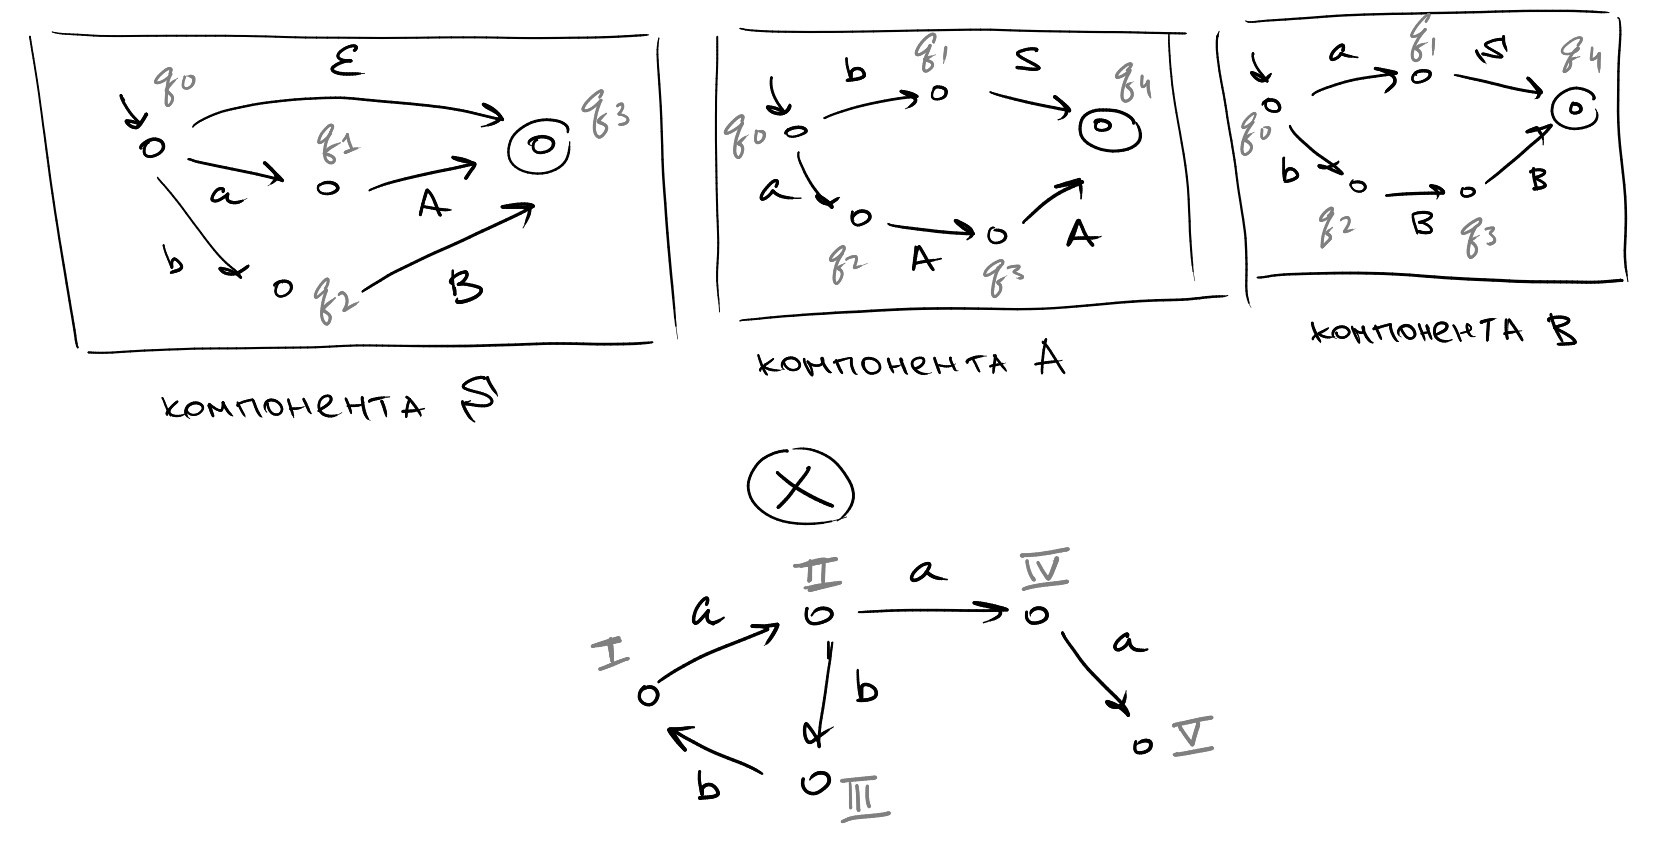
\includegraphics[width=1\linewidth]{img/example_intersection1}

%     \TODO: дорисовать пример (а потом перерисовать)

% \end{example}


\TODO: сделать на него ссылки везде (не только на него)

Все алгоритмы для CFPQ, которые будут описаны в этой работе имеют следующую схему:
\begin{enumerate}
    \item Построим прямое произведение входной грамматики $\cool{R}$ и входного графа $G$: $\cool{P} = \cool{R} \otimes G$.
    \item \textit{Решим задачу достижимости для полученного РКА $\cool{P}$}
    \item Из вершины $u$ в вершину $v$ входного графа существует путь, выводимой входной грамматикой $\cool{G}$ $\EQ$ в $\cool{P}$ есть путь из стартового состояния $(q_0, u)$ в конечное состояние $(q_f, v)$
\end{enumerate}

Рассмотрим внимательнее второй пункт~--- задачу достижимости для РКА. В случае обычного автомата эта задача эквивалентна задаче построения транзитивного замыкания~\cite{Yannakakis1990}. В случае же РКА задача осложняется наличием рекурсивных вызовов, которые разрешаются итеративно. (??)

\subsection{Алгоритм П}

В листинге~\ref{algo:P} приведён псевдокод Алгоритма П.

\TODO: что-то написать про епс-переходы

\begin{algorithm}[H]
    \floatname{algorithm}{Listing}
    \begin{algorithmic}[1]
    \caption{Алгоритм достижимости для РКА}
    \label{algo:P}
    \Function{RSMReachability}{$\cool{R}$}
        \State{$A \gets$ Adjacency matrix for $\cool{R}$}
        \While{$A$ is changing}
            \State{$A' \gets \textit{transitiveClosure}(A)$}
            \Comment{Построение транзитивного замыкания}
            \For{$i \in 1..k$}
               \For{$u \in En_i$}
                    \For{$v \in Ex_i$}
                        \If{$A'_{u,v} \wedge \overline{A_{u,v}}$}
                            \State{$A' \gets A' \cup getEdges(i, u, v)$}
                            \Comment{Добавление новых рёбер}
                        \EndIf
                    \EndFor
               \EndFor
            \EndFor
            \State{$A \to A'$}
        \EndWhile
    \State \Return $A$
    \EndFunction
    \end{algorithmic}
\end{algorithm}

Работа происходит над матрицей смежности $\cool{R}$~--- изначально туда записываются все ``внутренние'' (нерекурсивные) рёбра. 

Далее, внешний цикл повторяется, пока матрица смежности $A$ меняется (т.е. пока добавляются новые рёбра). На каждой итерации считается $A'$~--- транзитивное замыкание $A$. После этого находятся все новые пути вида $\langle$стартовое состояние$\rangle$ $\path$ $\langle$конечное состояние$\rangle$~--- те рёбра между стартовой и конечной вершинами компоненты, которых не было в $A$, но которые есть в $A'$~--- и добавляются соответствующие этим путям рёбра: для нового пути $(u \in En_i) \path (v \in Ex_i)$ проводятся все рёбра, соответствующие рекурсивным вызовам $i$-ой компоненты с начальной вершиной $u$ и конечной вершиной $v$.

\subsubsection{Пример}

\TODO

\subsubsection{Время работы}

Время работы~--- $k \cdot T(n)$, где $k$~--- число итераций внешнего цикла, $T(n)$~--- время работы одной итерации. 

Оценим $T(n)$. Внутренняя часть цикла состоит из двух частей: нахождения транзитивного замыкания (строка 4) и прохода по матрице для выявления новых рёбер (строки 5-9). 

Задача поиска транзитивного замыкания эквивалентна задаче перемножения булевых матриц~\cite{Aho1974} и может быть решена сведением к быстрому перемножению (обычных) матриц за $\O(n^\omega)$, где $2 < \omega < 2.273$~\cite{Alman20}.

Проход по матрице (строки 5-7) работает за $\O(n^2)$, что доминируется временем построения транзитивного замыкания. Добавление новых рёбер (строки 8-9) отработает суммарно за $\O(n^2)$ (т.к. каждое ребро будет добавлено не более одного раза).

Итого, время работы алгоритма $\O(k \cdot n^{\omega})$.

\subsection{Алгоритм П2}

Можно заметить, что не очень осмысленно на каждой итерации заново считать транзитивное замыкание, достаточно искать только пути, проходящие через рёбра, добавленные непосредственно на предыдущей итерации. То есть достаточно решать задачу {\bf инкрементального} транзитивного замыкания. 

В листинге~\ref{algo:P2} приведён псевдокод Алгоритма П2 (основанного на инкрементальном ТЗ)

\begin{algorithm}[H]
    \floatname{algorithm}{Listing}
    \begin{algorithmic}[1]
    \caption{Алгоритм достижимости для РКА (2)}
    \label{algo:P2}
    \Function{RSMReachability2}{$\cool{R}$}
        \State{$A \gets$ Empty adjacency matrix}
        \State{$Q \gets$ Empty Queue}
        \For{$i \in 1..k$}
            \For{$u \xrightarrow{c} v \in \delta_i$}
                \State{$Q.Push(\q{u, v, i})$}
            \EndFor
        \EndFor
        \While{$Q$ is not Empty}
            \State{$\q{u, v, i} \gets Q.Pop()$}
            \If{$u \in En_i \wedge v \in En_i$}
                \Comment{Нашли новый путь}
                \State{$A \gets A \cup getEdges(i, u, v)$}
                \State{$Q.PushAll(getEdges(i, u, v))$}
                \Comment{Добавляем новые рёбра}
            \EndIf
            \For{$x \in Q_i$}
                \If{$A_{x, u} \wedge \overline{A_{x, v}}$}
                    \For{$y \in Q_i$} 
                        \If{$A_{v, y} \wedge \overline{A_{x, y}}$}
                            \State{$A \gets A \cup \q{x, y}$}
                            \State{$Q.Push(\q{x, y, i})$}
                            \Comment{Обновлем транзитивное замыкание}
                        \EndIf
                    \EndFor
                \EndIf
            \EndFor
        \EndWhile
    \State \Return $A$
    \EndFunction
    \end{algorithmic}
\end{algorithm}

В алгоритме используется (более менее) стандартная реализация инкрементального транзитивного замыкания~\cite{Ibaraki1983}. Для этого в ходе работы алгоритма поддерживается рабочая очередь $Q$ рёбер транзитивного замыкания, которые были найдены, но ещё не обработаны. 

При обработке очередного \textit{(потому что оно из очереди ахахах)} ребра, ищутся новые пути, которые проходя через него. А именно, пусть было добавлено ребро $u \to v$. Тогда далее перебирается вершина $x$, такая что из неё была достижима вершина $u$ ($x \path u$), но не была достижима вершина $v$ ($x \not\path v$). Из такой вершины $x$ становятся достижимы все вершины $y$, которые были достижимы из $v$ ($v \path y$).

Также, как и в Алгоритме П, если ребро ТЗ (= путь в графе) соединяет начальную и конечную вершину, в очередь добавляются также все соответствующие ему рекурсивные рёбра.

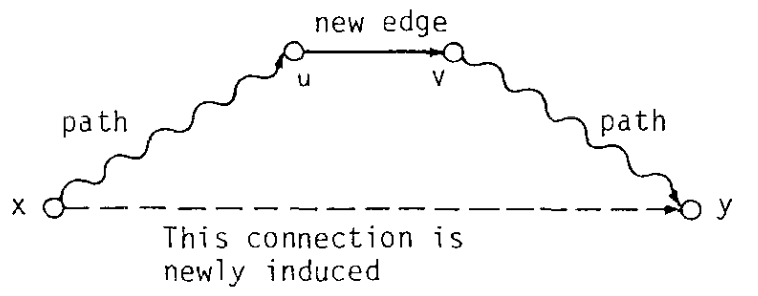
\includegraphics[width=0.75\linewidth]{img/TC_add}

\TODO: норм картинка

\subsubsection{Время работы}

Внешний цикл итерируется по всем рёбрам, так что работает за $\O(m^{*})$. Добавление новых рёбер как и в алгоритме П рассмотрит каждое ребро не более одного раза, так что тоже работает за $O(m^{*})$. Нужно только оценить работу по поддержанию транзитивного замыкания. 

Цикл на строке 12 перебирает все вершины, так что отработает суммарно за $\O(m^{*} n)$. Внутренний цикл (строка 14) тоже перебирает все вершины, но после его выполнения будет добавлено хотя бы одно новое ребро ($x \to v$), так что суммарное время работы этих циклов также можно оценить как $\O(m^{*} n)$.

Итого, суммарное время работы составляет $\O(n m^{*})$, что в плотных графах будет равно $\Theta(n^3)$. 

\begin{note}
Время работы итеративного транзитивного замыкания можно ускорить в $\log n$ раз~\cite{Chaudhuri08}, воспользовавшись методом четырёх русских~\cite{Arlazarov70} (так как работа происходит над булевыми векторами).
\end{note}

\subsection{Загадка дыры}

Основой для получения частных решений будут модификации Алгоритмов П и П2.

{\bf Модифицируем Алгоритм П2}

Как уже было сказано, узким местом Алгоритма П2 является построение инкрементального транзитивного замыкания, которое в общем случае нельзя (скорее всего) решить быстрее, чем за кубическое время.

Следовательно, чтобы получить более быстрый алгоритм в частном случае, нужно рассматривать такие частные случаи, для которых задачу инкрементального транзитивного замыкания можно решать быстрее.

Рассмотрим сначала всякие несложные случаи:

\begin{itemize}
    \item Графы с ограниченной степенью

    В~\cite{Yellin1993} представлен алгоритм для инкрементального транзитивного замыкания на графах с ограниченной исходящей степенью. Асимптотика алгоритма: $\O(d m^{*})$, где $d$~--- ограничение сверху на исходящую степень графа, а $m^{*}$~--- число рёбер в транзитивном замыкании.
    \item Планарные (?)

    \TODO: Разобраться, что там написала Александра 
    
    \item Bounded-stack SM 

    % $\O(n^3 k^3 / \log^2)$ \cite{Chaudhuri08}

%         RSM, который не уходит в рекурсию (т.е. есть из конца ребра $\xrightarrow{S}$ не достижимо никакое ребро $\xrightarrow{S}$)

%         Тут применяется какое-то более хитрое (я ещё не разбиралась) итеративное транзитивное замыкание (что-то с dfs'ом, а потом ещё 4 русских сверху, кажется)

    \item Неориентированные графы


    Вот тут получаем нетривиальные результаты, про них в следующем разделе
\end{itemize}

% https://www.sciencedirect.com/science/article/pii/0304397586900988
% O(n) amortized per edge

% Так что, чтобы получить полиномиальное ускорение, нужно как-то ослабить условия, в которых решается задача построения итеративного транзитивного замыкания. 

\subsection{Выводы и результаты по главе}

\TODO
